\section{Patrones de diseño y arquitectónicos}
En este apartado se procederá a explicar los diferentes patrones de diseño y de arquitectura presentes en el proyecto.

\subsection{Patrones arquitectónicos}
Los patrones arquitectónicos \cite{Dessign_patterns} son aquellos que se encargan de dar una estructura esencial al proyecto con un nivel de abstracción mucho mayor a los patrones de diseño.

\subsubsection{\textbf{Modelo Vista Presentador (MVP)}}
\begin{figure}[H]
    \centering
    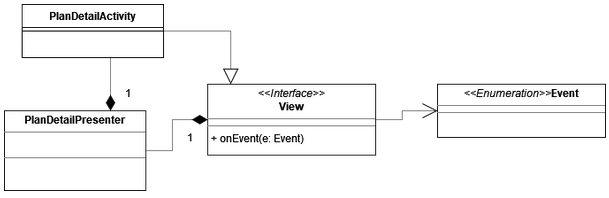
\includegraphics[width=\textwidth]{Images/Capitulo6/modelomvp.png}
    \caption{Esquema de Modelo Vista Presentador}
    \label{fig:esquemamvp}
\end{figure}

El patrón MVP (Modelo-Vista-Presentador) es un patrón de arquitectura principalmente utilizado para generar interfaces de usuario. Como se puede apreciar en la figura \ref{fig:esquemamvp}, este patrón encapsula toda la lógica de la vista a través del presentador, recogiendo los datos del propio modelo del sistema.
Es un diseño arquitectónico muy utilizado para la realización de aplicaciones Android o aplicaciones web desarrolladas mediante el lenguaje de programación ASP.NET.
En modelo vista presentador, nos podemos encontrar tres diferentes elementos:
\begin{itemize}
    \item \textbf{Modelo}: interfaz que define los datos y la estructura de los mismos.
    \item \textbf{Presentador}: clase mediadora entre la vista y el modelo. Es la encargada de actualizar los datos de la vista recogidas desde el modelo y actualizar el modelo con los datos recibidos de la vista.
    \item \textbf{Vista}: interfaz que muestra los datos obtenidos del presentador. Lo que el usuario ve al abrir la aplicación.
\end{itemize}

\subsection{Patrones de diseño}
Los patrones de diseño son unas técnicas para resolver problemas comunes en el desarrollo de software referentes al diseño de interacción o interfaces. Un patrón de diseño resulta ser una solución a un problema de diseño.
\subsubsection{\textbf{Singleton}}
\begin{figure}[H]
    \centering
    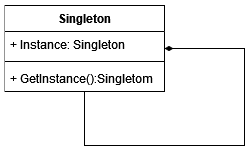
\includegraphics[width=0.5\textwidth]{Images/Capitulo6/singleton.png}
    \caption{Esquema del patrón Singleton}
    \label{fig:singleton}
\end{figure}
El patrón Singleton (fig \ref{fig:singleton}) es utilizado para garantizar una única instancia del objeto al que queremos acceder, haciendo el código más eficiente. Por cada referencia al uso de la clase, se proporciona un único punto de acceso a la instancia llamando al método \texttt{getInstance()}, el cual devuelve la instancia o la crea si antes no se ha llamado a dicho método.

Este patrón se ha usado en la aplicación Android para hacer única la capa de servicios de la aplicación encargada de la creación, principalmente, de los modelos correspondientes.
La base de datos de Firebase también está creada mediante este patrón, teniendo una única instancia de referencia a la base de datos.

\subsubsection{\textbf{Façade}}
\begin{figure}[H]
    \centering
    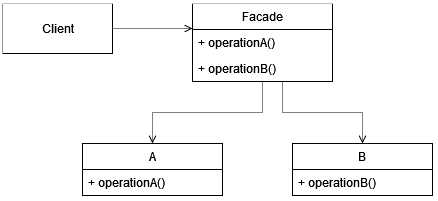
\includegraphics[width=0.75\textwidth]{Images/Capitulo6/facade.png}
    \caption{Esquema del patrón Façade}
    \label{fig:facade}
\end{figure}
El Patrón Façade o patrón Fachada (fig \ref{fig:facade}) proporciona una interfaz unificada para un conjunto de interfaces del subsistema ocultando al cliente los componentes del subsistema, reduciendo el número de objetos que accede el cliente.
En este proyecto se ha utilizado este patrón para unificar las diferentes llamadas a las diferentes API generadas para la realización de este proyecto.

\subsubsection{\textbf{Adapter}}
\begin{figure}[H]
    \centering
    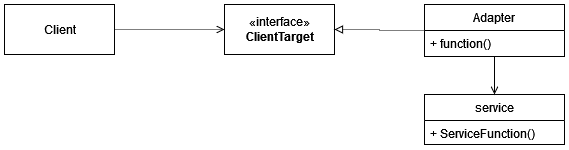
\includegraphics[width=\textwidth]{Images/Capitulo6/adapter.png}
    \caption{Esquema del patrón Adapter}
    \label{fig:adapter}
\end{figure}
El patrón Adaptador (fig \ref{fig:adapter}) es el encargado de convertir la interfaz de un objeto para que otro objeto pueda comprenderla.
Es por ello que se ha implementado este patrón para adaptar los productos obtenidos mediante la API haciéndolas un objeto entendible para el cliente. 
Otro de los motivos para los que se ha propuesto dicho patrón es para la creación de listas dinámicas en cada una de las vistas necesarias. Estas vistas se han desarrollado mediante el elemento \texttt{RecyclerView} propio de Android en el que mediante un adaptador se implementan las diferentes listas u objetos adaptados para que el cliente pueda observarlas con mayor claridad.

\subsubsection{\textbf{Transfer}}
\begin{figure}[H]
    \centering
    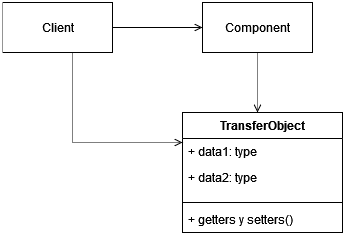
\includegraphics[width=0.6\textwidth]{Images/Capitulo6/transfer.png}
    \caption{Esquema del patrón Transfer}
    \label{fig:transfer}
\end{figure}
El patrón Transfer (fig \ref{fig:transfer}) es el encargado de agrupar varios datos en una misma clase facilitando el intercambio de información entre las diferentes capas del proyecto.

En este proyecto se ha utilizado el patrón para el propio propósito, para mostrar datos al usuario y para insertarlos a la propia base de datos.

\subsubsection{\textbf{View helper (ayudante de vista)}}
\begin{figure}[H]
    \centering
    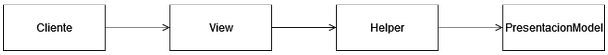
\includegraphics[width=\textwidth]{Images/Capitulo6/view.png}
    \caption{Esquema del patrón View Helper}
    \label{fig:view}
\end{figure}
El patrón View Helper o ayudante de vista (fig \ref{fig:view}) se encarga de la creación de la vista mejorando la partición, reutilización y mantenibilidad de la misma separando los roles y facilitando la prueba.
En este proyecto el patrón se utiliza con la utilización del \texttt{RecyclerView} de la plataforma Android, delegando toda la lógica de las listas dinámicas y su funcionamiento a la clase Adapter que necesita para generar la vista dinámica.